\section{Object Detection Metrics}
\subsection*{Task 1a}
When talking about precision metrics, Intersection over Union can be useful to mention.
Especially when we want to mesure how well a neural network is able to separate objects by using bounding boxes.
In intersection over union we measure how much of the predicted bounding box overlaps with the ground truth, being the real bounding box.
For illustrating this even further, I have drawn to boxes in a figure below. 
As we can see in the illustration, we have one red box behind a blue box. 
The intersection between them is illustrated by the color purple. 
To measure the prediction of the bounding box, we take the intersection of the two boxes (purple area), divided by the union of the two boxes (red and blue).

\begin{equation*}
    IoU = \frac{\text{area of overlap}}{\text{area of union}}
\end{equation*}

\begin{figure}[h!]
    \centering
    
\includegraphics[width=0.8\textwidth]{Images/task1a.png}
    \caption{Intersection over Union}
\end{figure}

\subsection*{Task 1b}
In this subsection we will introduce the two performance metrics \textbf{Precision} and \textbf{Recall}.
The metrics are built up by different shares of \textit{True} and \textit{False} \textit{Positives} and \textit{Negatives}, and the defintions of these should be known before we introduce the equations.
A \textbf{True Positive (TP)} is that we have predicted the result as a positive, agreeing with the ground truth and being a correct prediction.
A \textbf{True Negative (TN)} is that we have correctly predicted the result to be negative.
A \textbf{False Positive (FP)} is an incorrect predition, where we have predicted it to be positive, but the truth is that it is negative.
And last, but not least, we have a \textbf{False Negative (FN)} which is that we have incorrectly predicted the result to be negative, when it actually is positive.
Then we are ready for the formulas.

\paragraph{Precision} How many of the positive predictions we have made are correct?
\begin{equation*}
    Precision = \frac{TP}{TP + FP}
\end{equation*}
\paragraph{Recall} How well are we able to find all the positives there is?
\begin{equation*}
    Recall = \frac{TP}{TP + FN}
\end{equation*}

\subsection*{Task 1c}
We are tasked to find the mean average precision between two precision-recall curves.
I start off by plotting each of the given curves and calculate the Average Precision.
Then we can calculcate the Mean Average Precision (mAP).

The average precision is calculated using the following equation

\begin{equation*}
    AP = \frac{1}{\text{number of points}} \displaystyle\sum_{r \in \{0.0,...,1.0\}}  Precision
\end{equation*}

One thing to mention here is that the number of points is 11, being the elements $$\{0.0, 0.1, 0.2, 0.3, 0.4, 0.5, 0.6, 0.7, 0.8, 0.9, 1.0\}$$
For calculating the average precision we sum the precision at each of these points and divide by the total number of points for averaging.


The mean average precision can then be calculated with the following equation

\begin{equation*}
    mAP = \frac{1}{\text{number of APs}}\;\frac{\text{sum of APs}}{\text{number of points in AP}}
\end{equation*}


For this task, I wanted to test out another aspect as well. 
Earlier, when calculating average precision, we have used interpolation.
Therefore, I want to calculate the mAP with both an interpolated and non-interpolated curve in this task, for comparing the different results.

The task continue on the next page.

\clearpage

\begin{figure}[h!]
    \centering
    \begin{subfigure}[b]{0.24\textwidth}
        \centering
        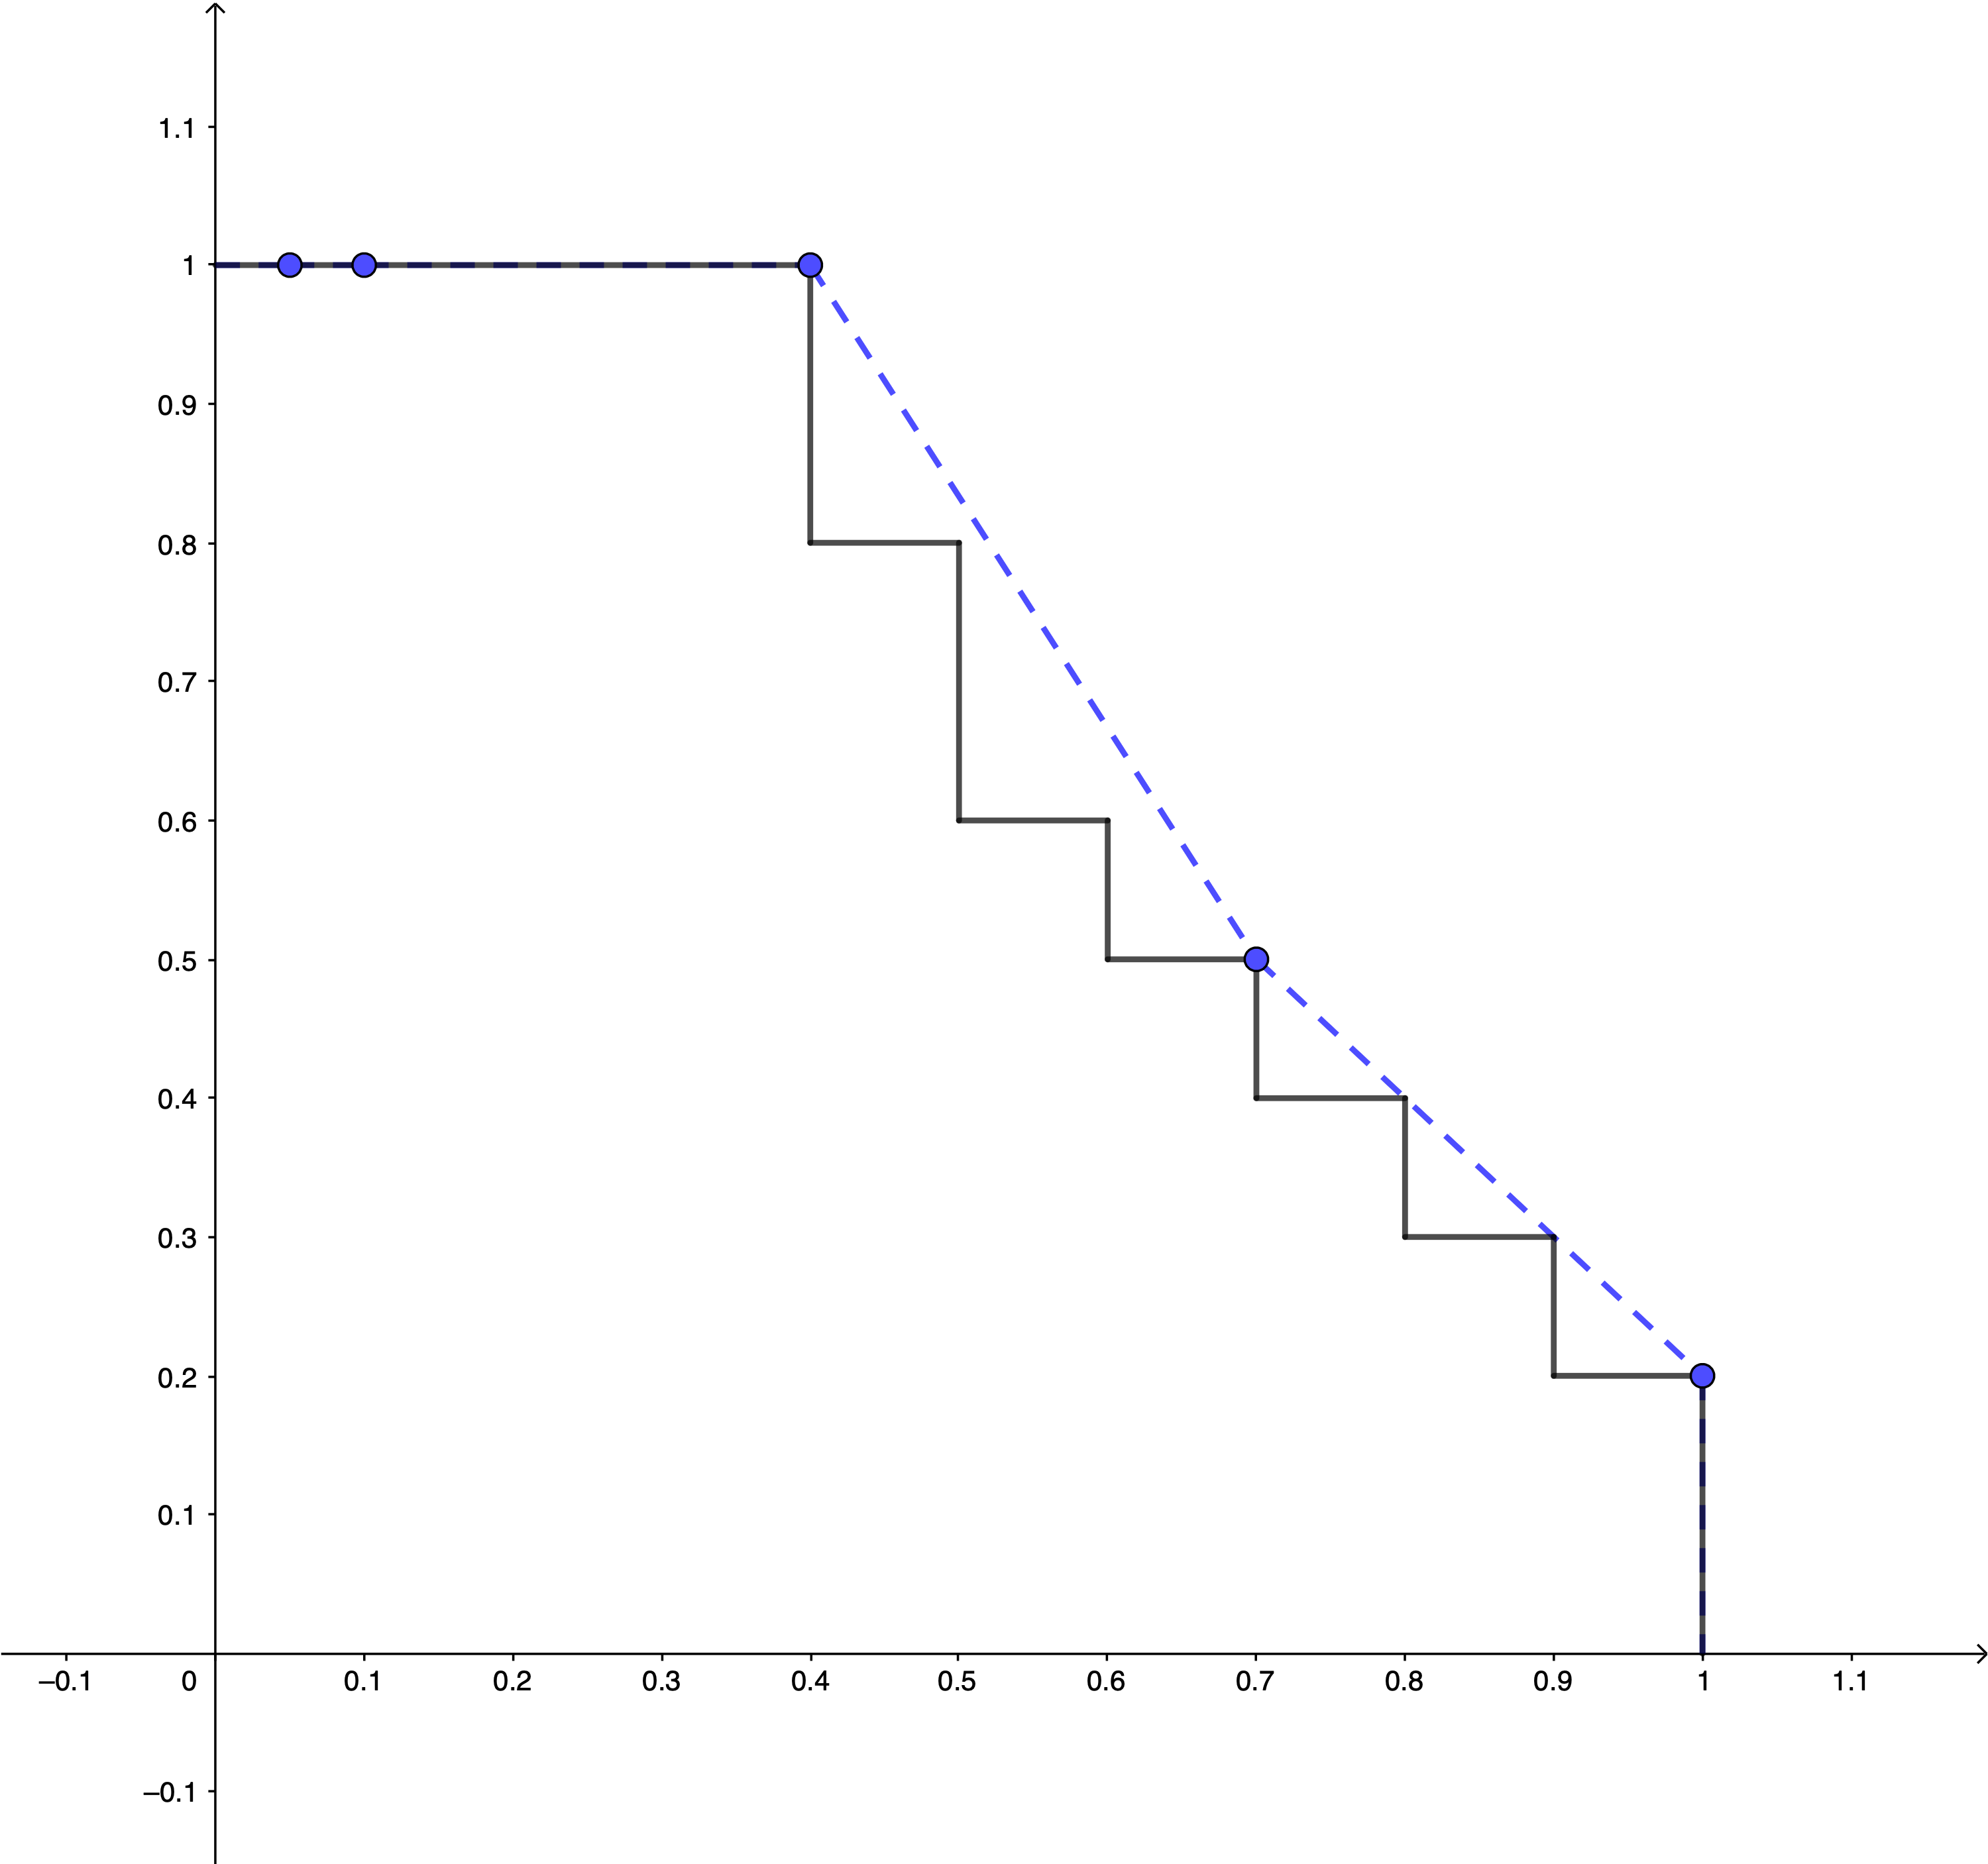
\includegraphics[width=\textwidth]{Images/task1c1.png}
        \caption*{Class 1}
    \end{subfigure}
    \hfill
    \begin{subfigure}[b]{0.24\textwidth}
        \centering
        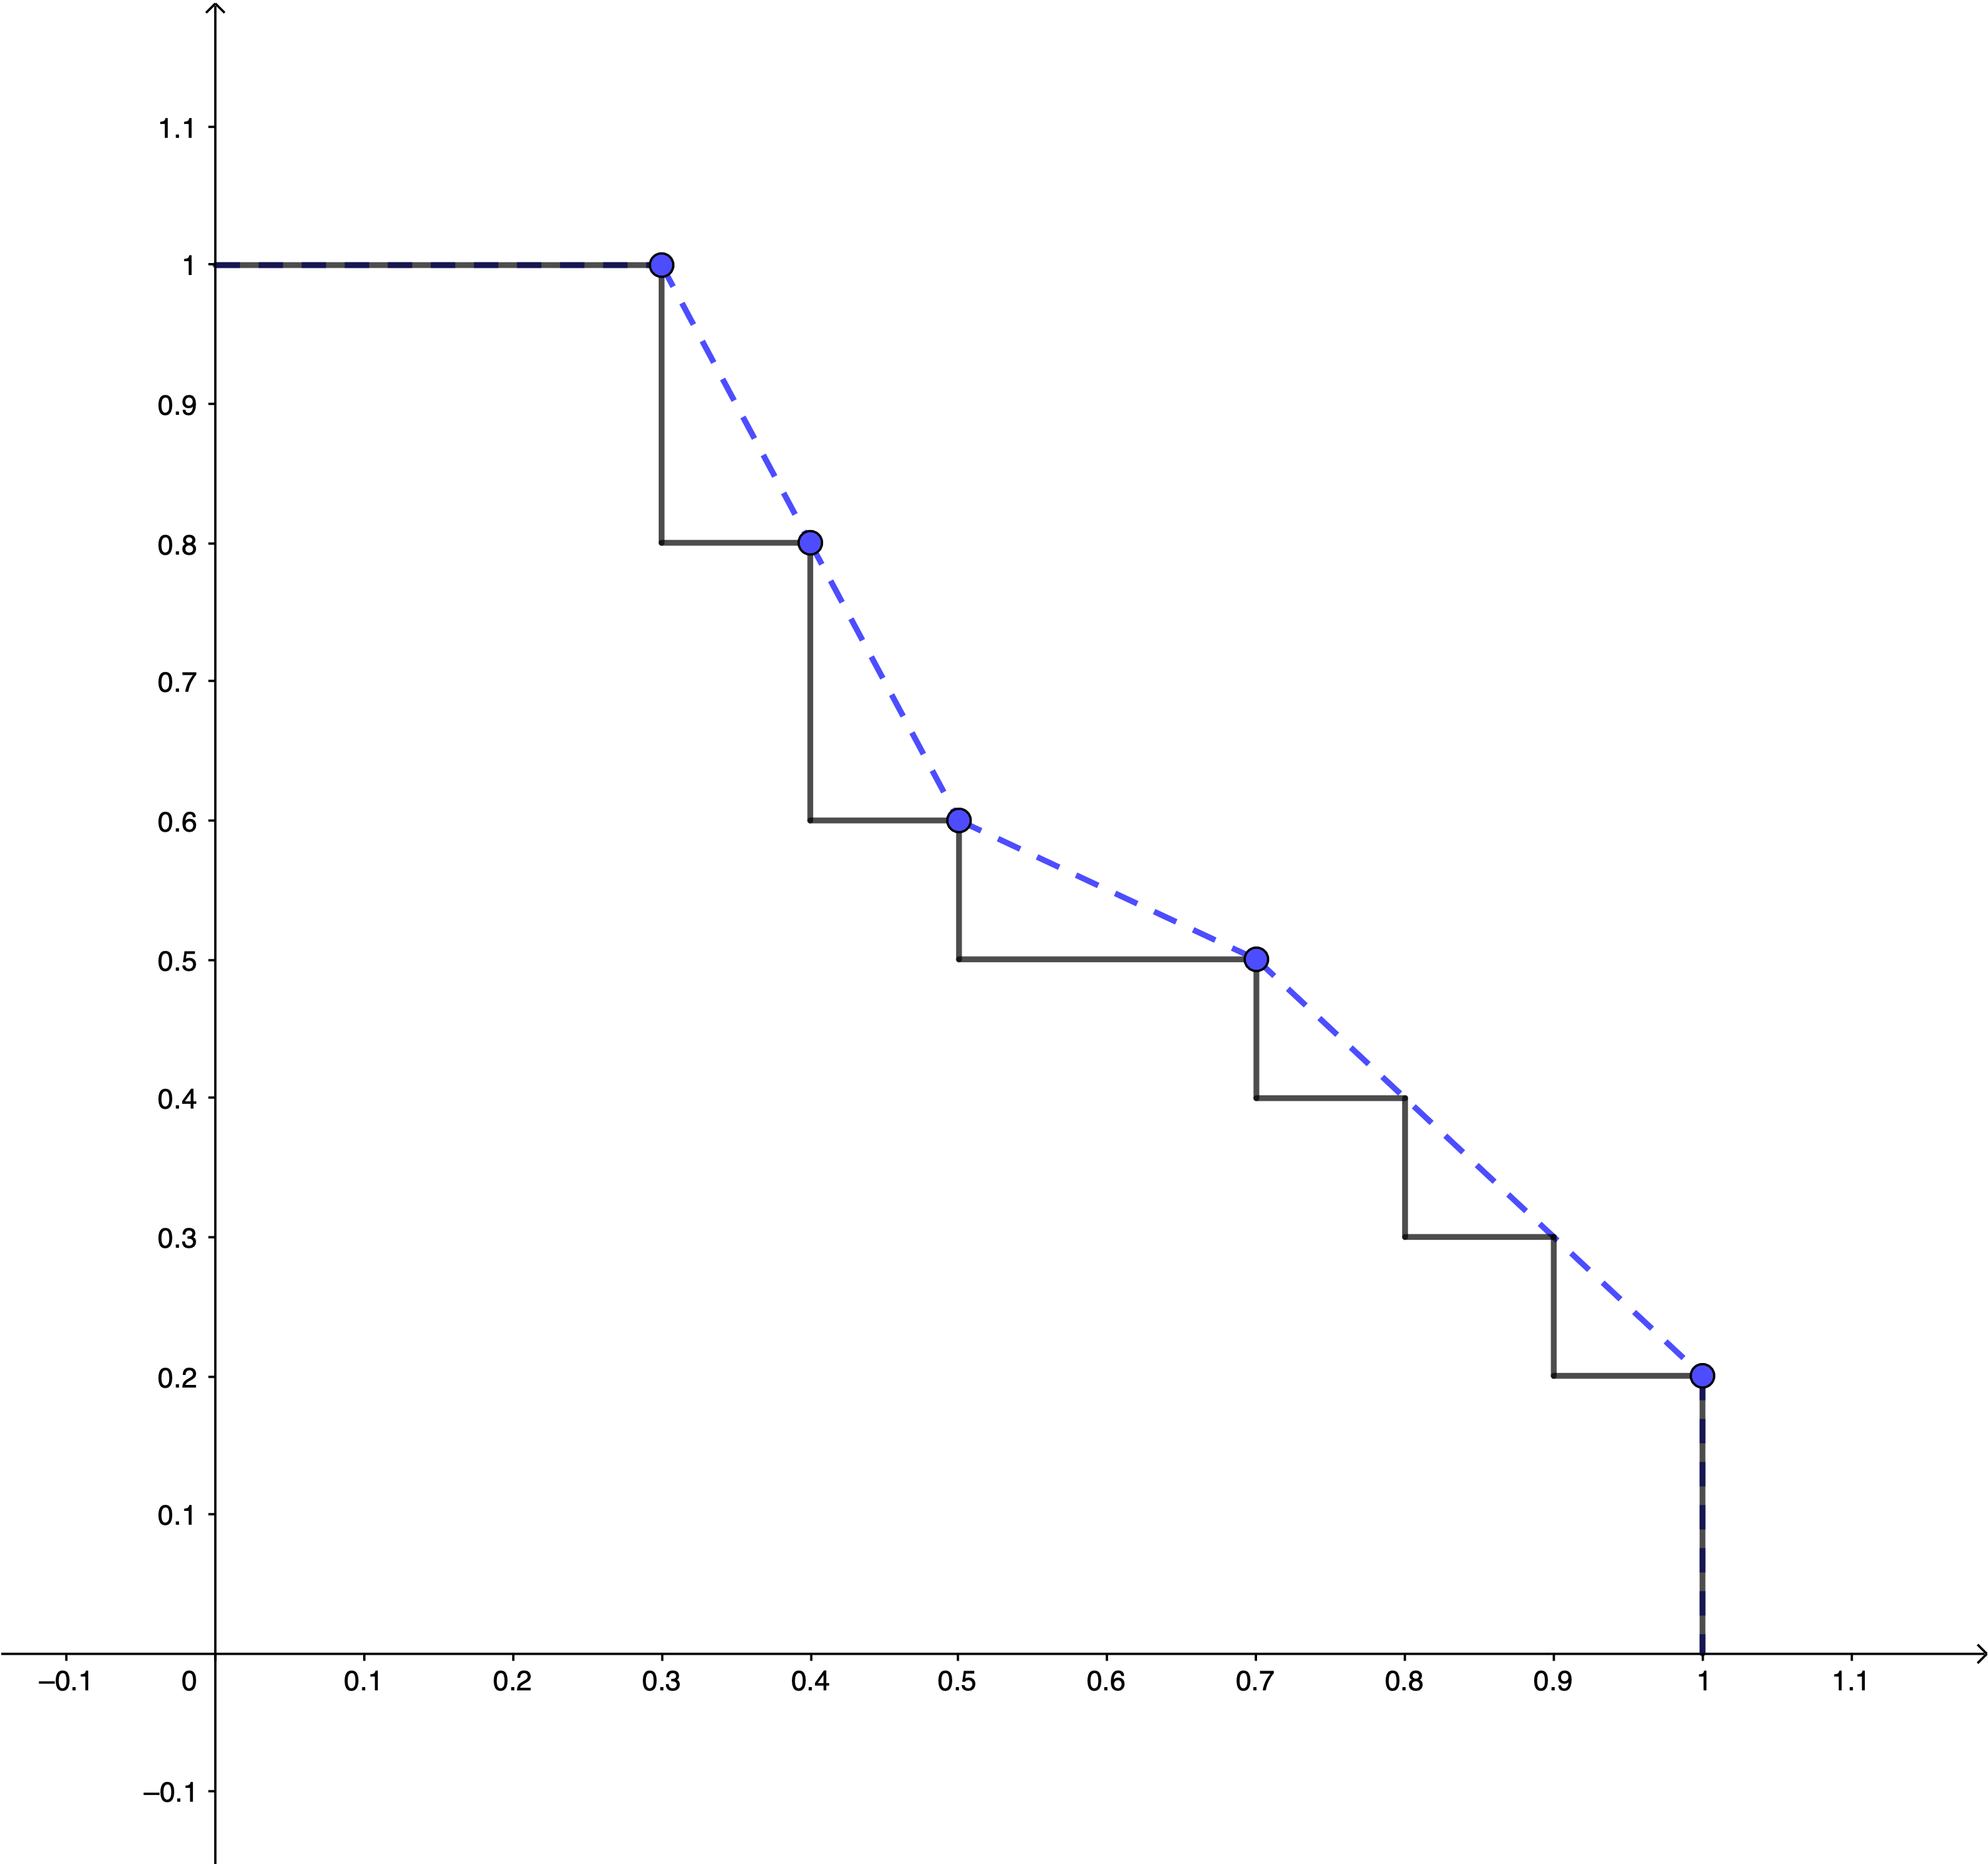
\includegraphics[width=\textwidth]{Images/task1c2.png}
        \caption*{Class 2}
    \end{subfigure}
    \hfill
    \begin{subfigure}[b]{0.24\textwidth}
        \centering
        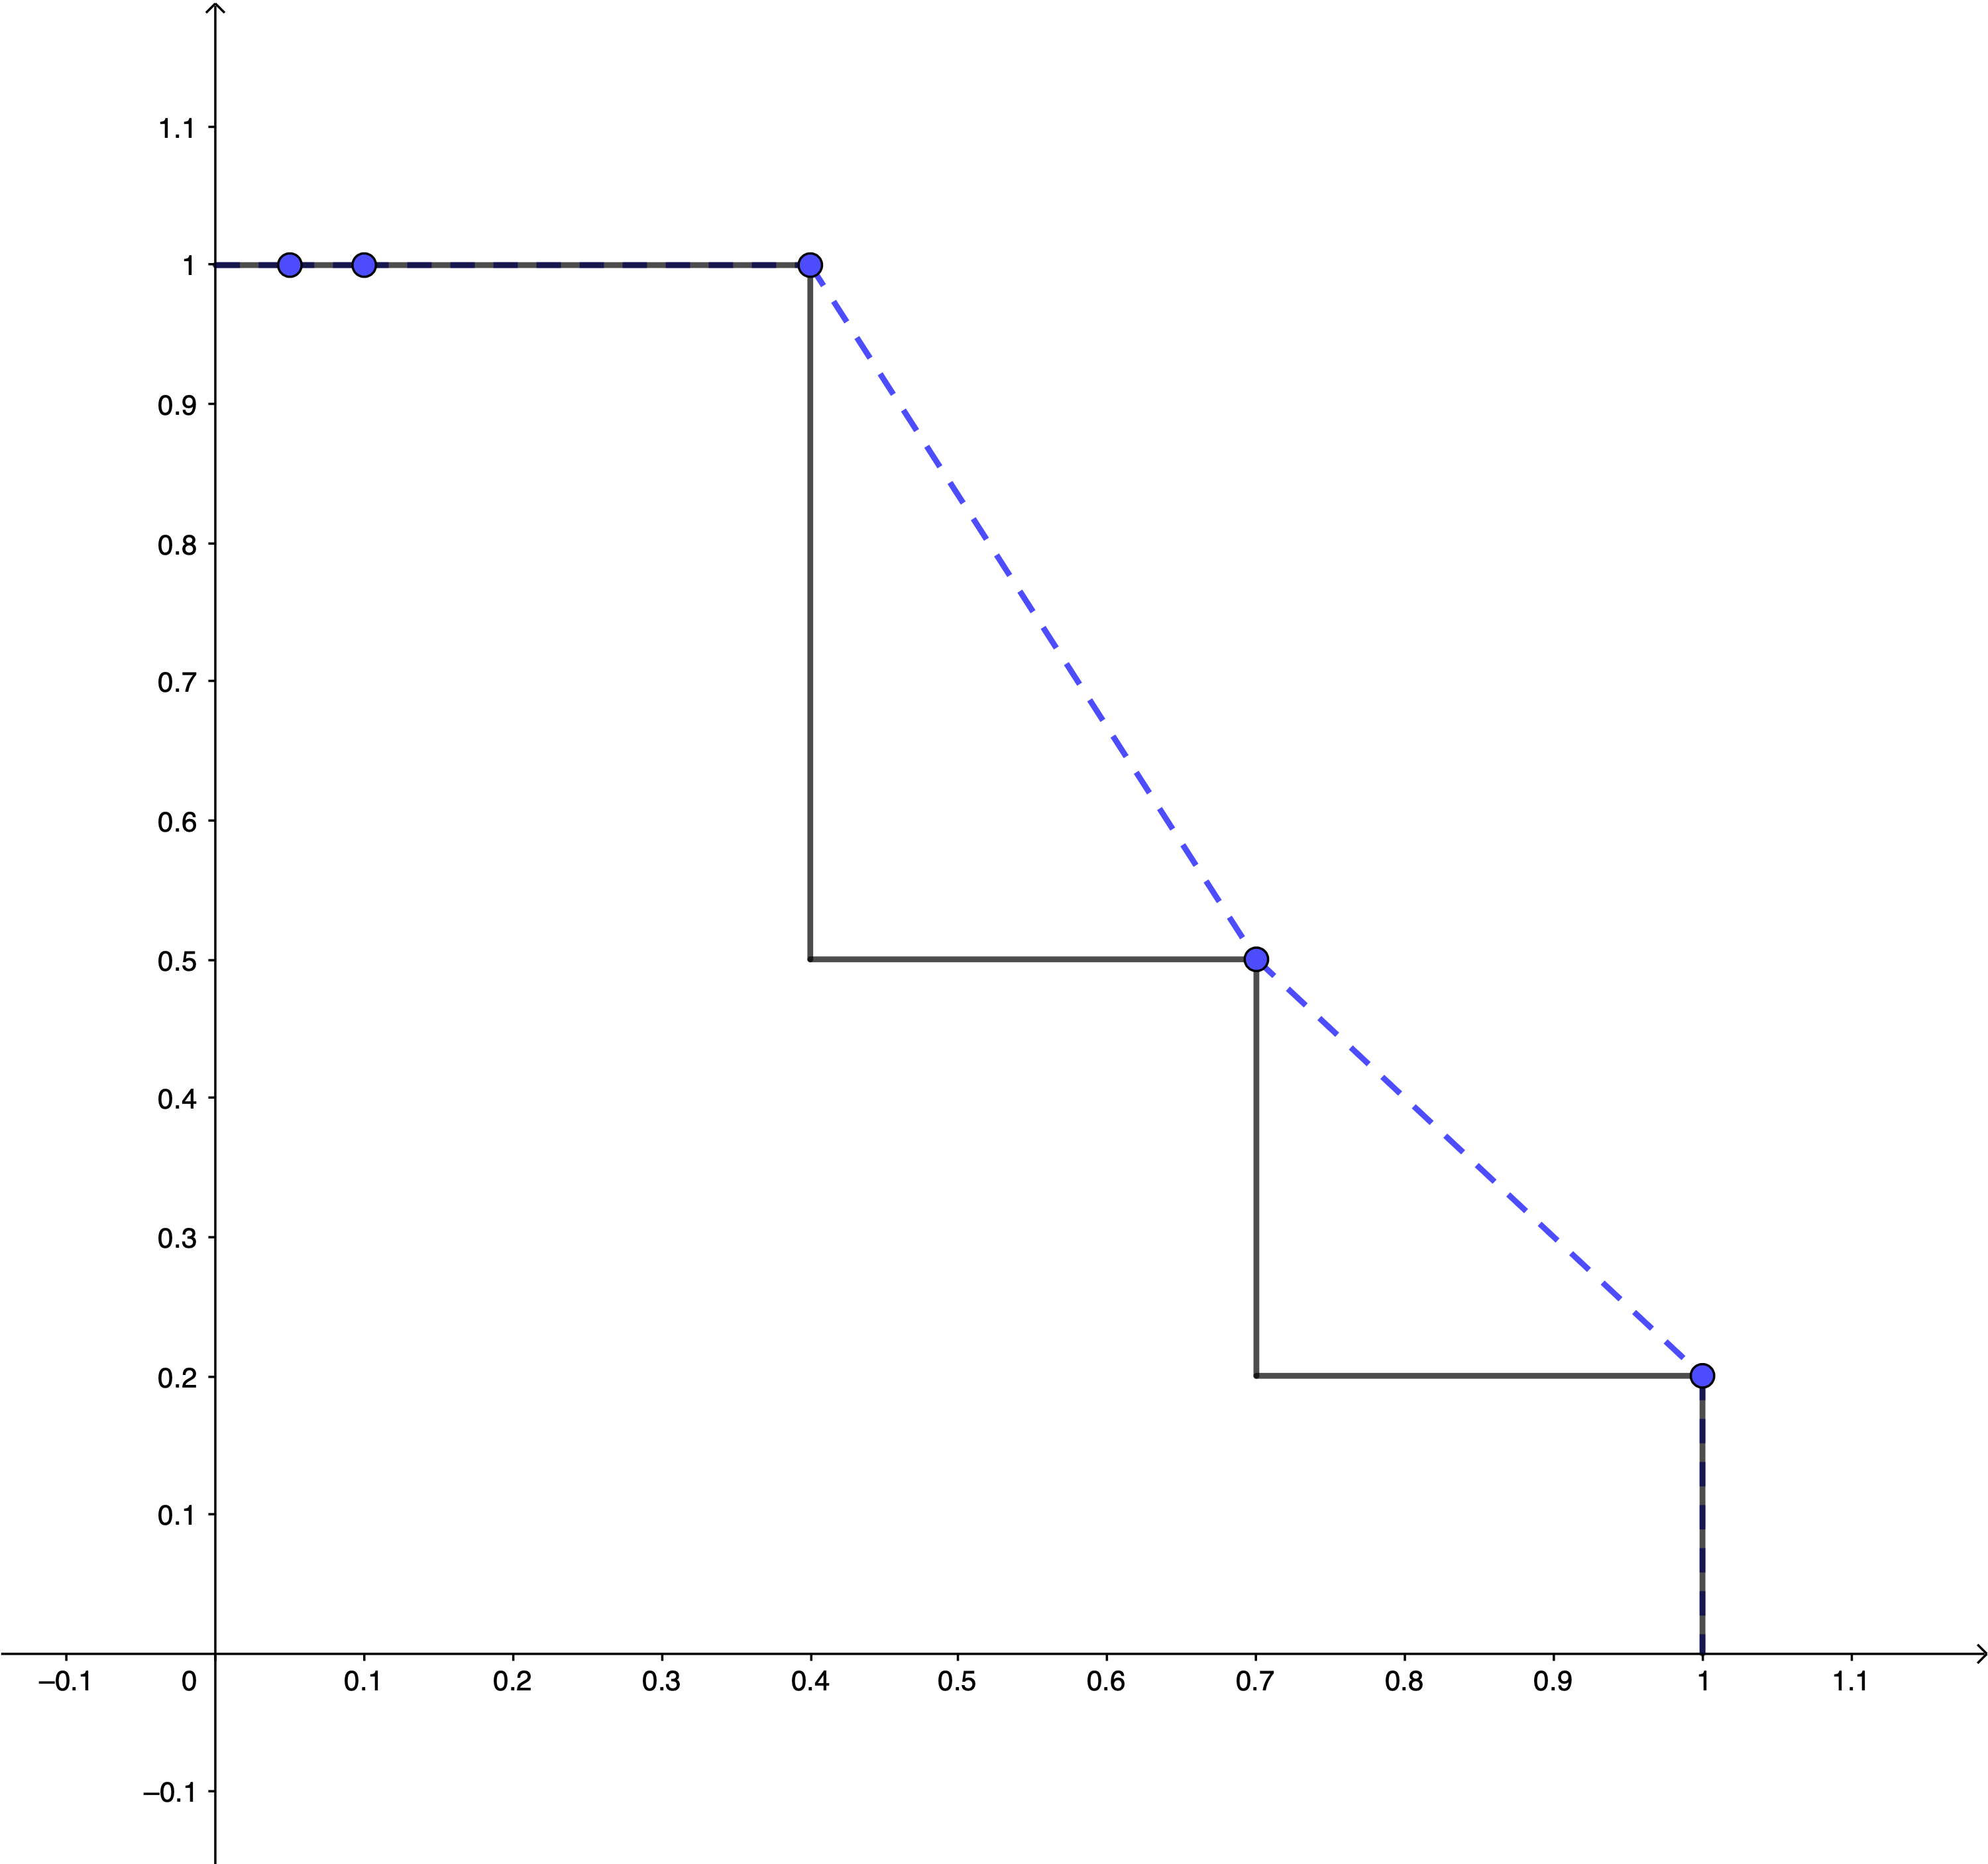
\includegraphics[width=\textwidth]{Images/task1c1_interpolated.png}
        \caption*{Class 1 interpolated}
    \end{subfigure}
    \hfill
    \begin{subfigure}[b]{0.24\textwidth}
        \centering
        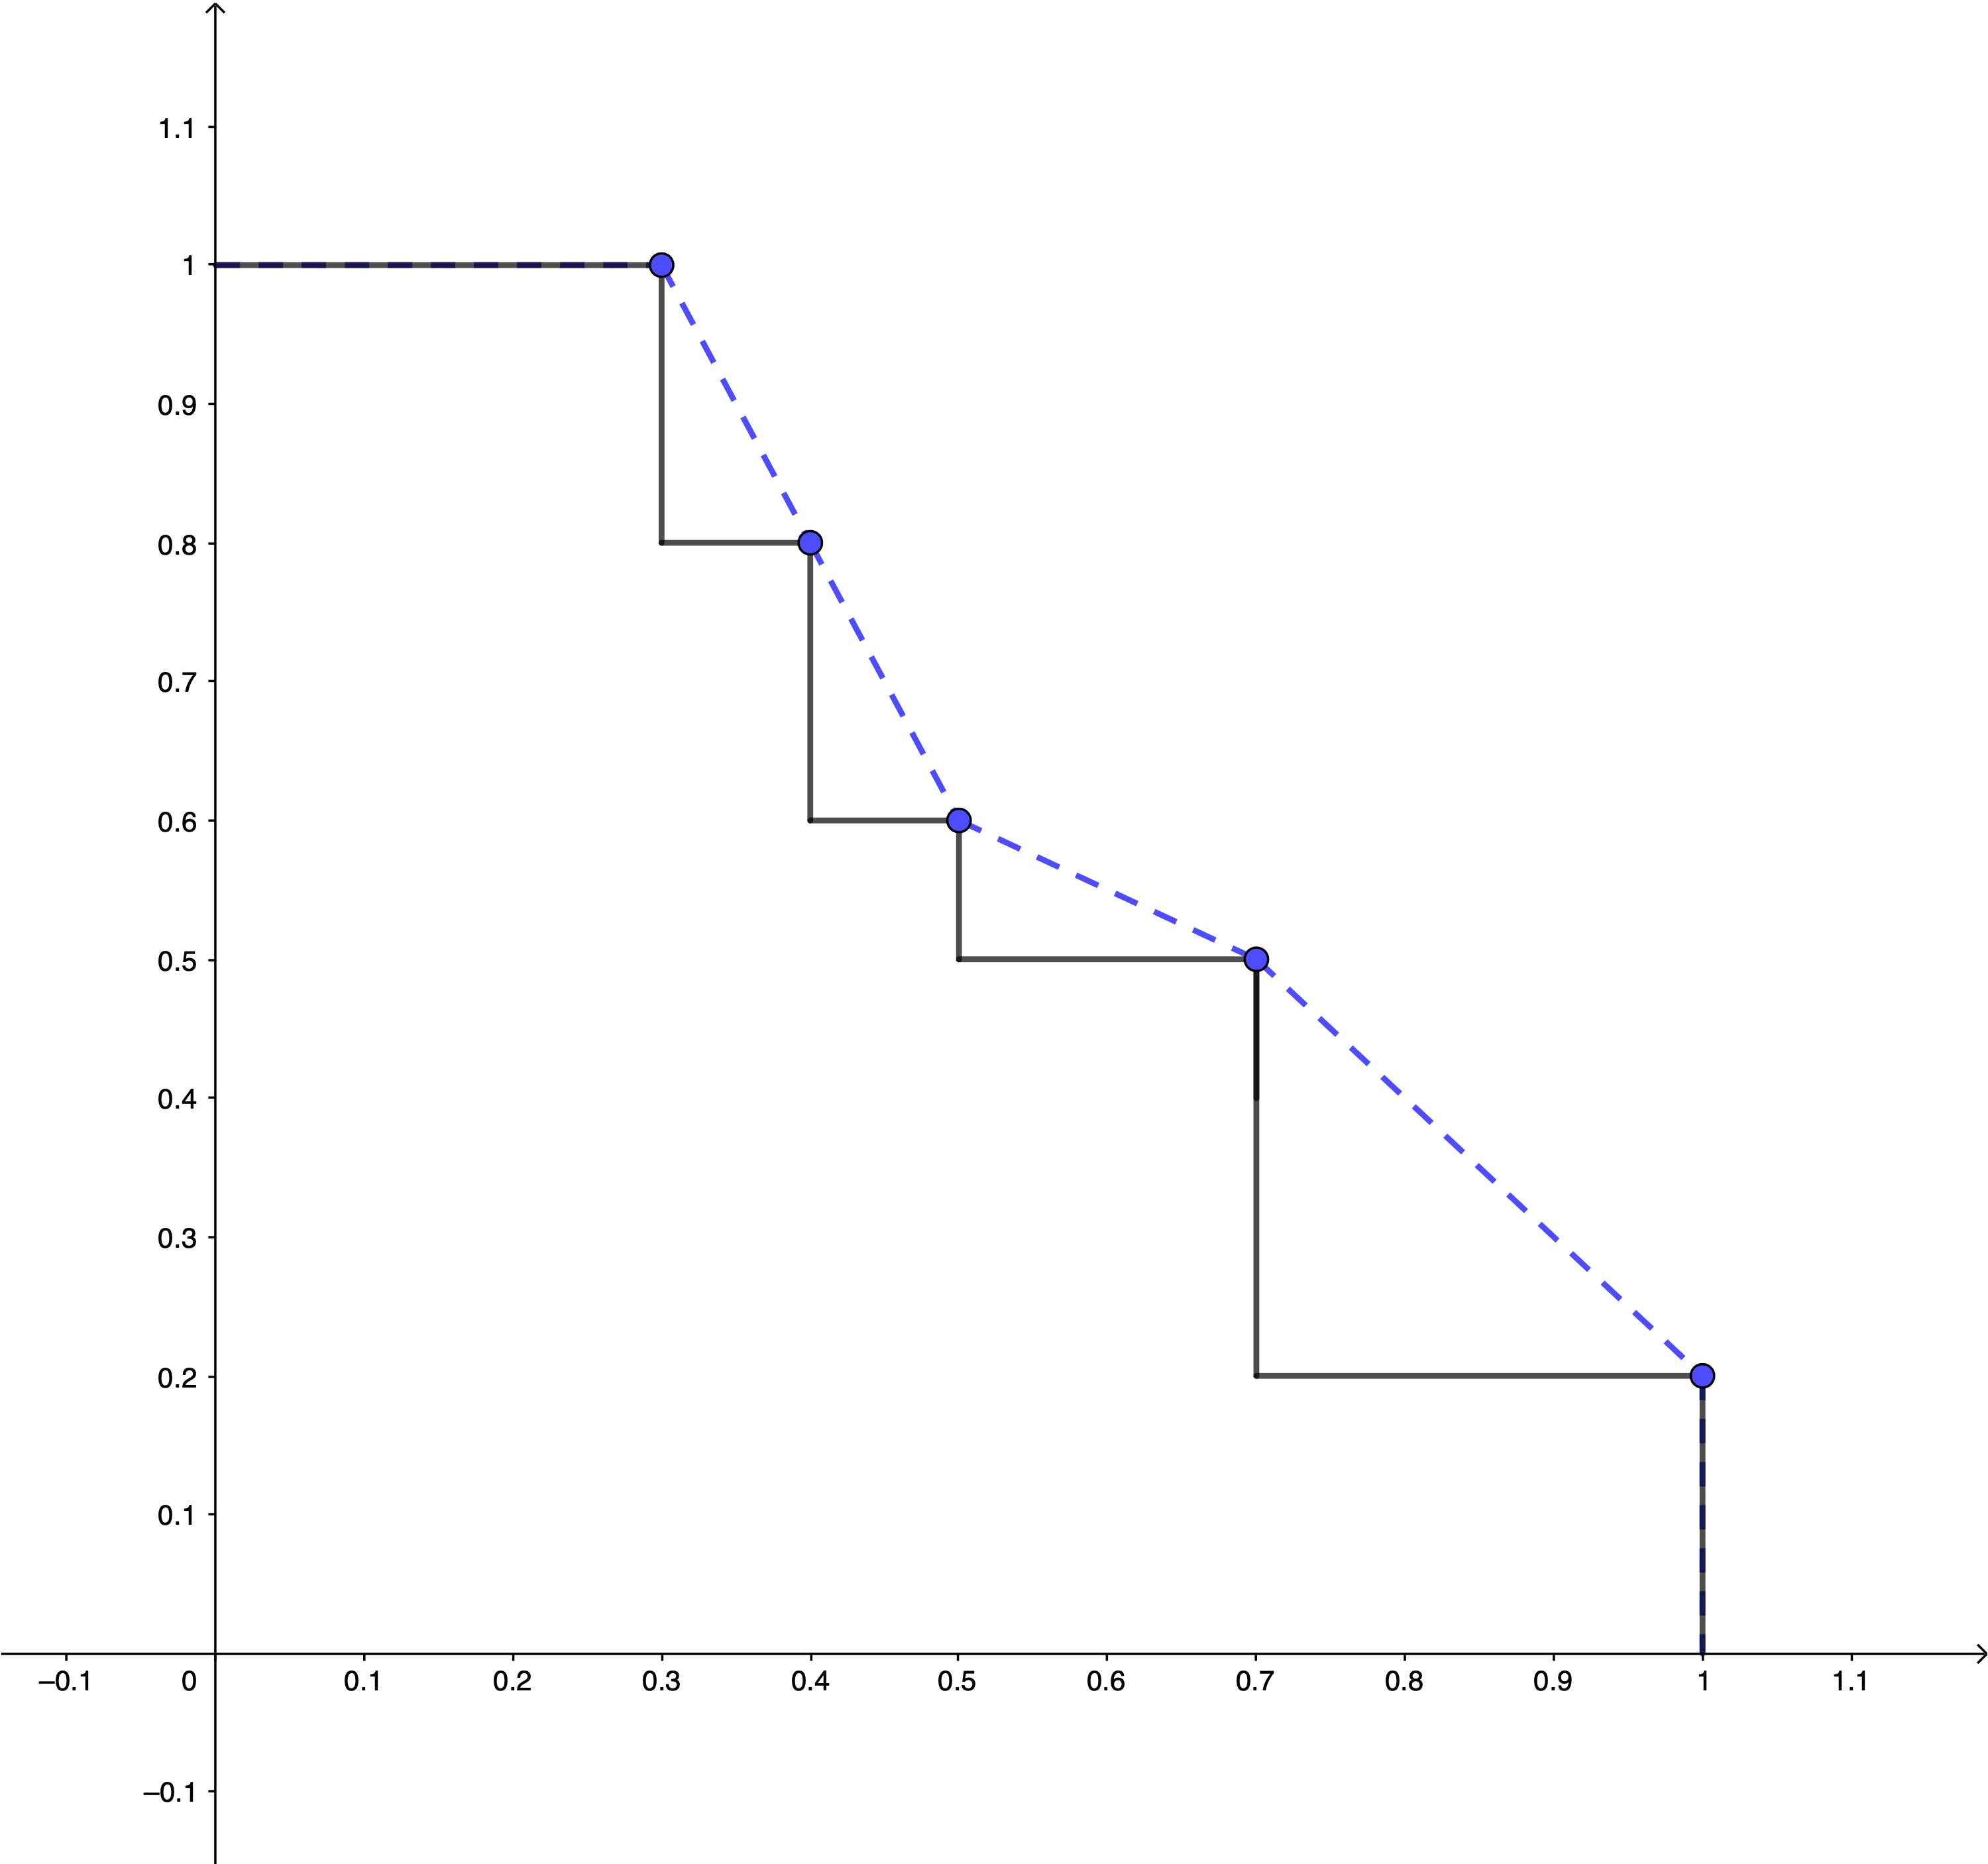
\includegraphics[width=\textwidth]{Images/task1c2_interpolated.png}
        \caption*{Class 2 interpolated}
    \end{subfigure}
    \caption{Plots of classes, both original and interpolated}
\end{figure}

\subsubsection*{Original}

Class 1 yields the following average precision
\begin{equation*}
    AP = \frac{1}{11}(5*1.0+0.8+0.6+0.5+0.4+0.3+0.2) = \frac{7.8}{11} = 0.709
\end{equation*}

Class 2 yields the following average precision
\begin{equation*}
    AP = \frac{1}{11}(4*1.0+0.8+0.6+2*0.5+0.4+0.3+0.2) = \frac{7.3}{11} = 0.664
\end{equation*}

Which altogether gives a mean average precision of
\begin{equation*}
    mAP = \frac{1}{2}\frac{7.8+7.3}{11} = 0.686
\end{equation*}

\subsubsection*{Interpolated}

Class 1 yields the following average precision
\begin{equation*}
    AP = \frac{1}{11}(5*1.0+3*0.5+3*0.2) = \frac{7.1}{11} = 0.645
\end{equation*}

Class 2 yields the following average precision
\begin{equation*}
    AP = \frac{1}{11}(4*1.0+0.8+0.6+2*0.5+3*0.2) = \frac{7}{11} = 0.636
\end{equation*}

Which altogether gives a mean average precision of
\begin{equation*}
    mAP = \frac{1}{2}\frac{7.1+7}{11} = 0.641
\end{equation*}

Which shows that the original and interpolated mAP show some variations, though not too much.
One may still prefer the original one, but one thought would be to have accurate measures at each point, which could have made it even more precise.










